
\subsection{Answers}
\begin{table}[htb]%
\begin{center}%
\caption{Q19: What are your obstacles to mastering MPI?}%
\label{tab:Q19-ans}%
\begin{tabular}{l|l|r}%
\hline%
Choice & Abbrv. & \# Answers \\%
\hline%
I have no obstacles. & No obstacles & 332 (41.3\%) \\%
Too many routines. & Too many routines & 169 (21.0\%) \\%
Too complicated and hard to understand. & Complicated & 115 (14.3\%) \\%
No appropriate lecture / book / info. & No appropriate one & 110 (13.7\%) \\%
I have nobody to ask. & Nobody to ask & 83 (10.3\%) \\%
I do not like the API. & Dislike API & 68 (8.5\%) \\%
other & - & 111 (13.8\%) \\%
\hline%
\multicolumn{2}{c}{total} & 988 (803)\\%
\hline%
\end{tabular}%
\end{center}%
\end{table}%


\subsection{List of other answers}
\begin{itemize}
\item Africa: I am too busy
\item Central and South America: the message passing paradigm
\item Europe:France: Difficulty to debug
\item Europe:France: Efficient debugging knowledges
\item Europe:France: Have not kept up with recent changes
\item Europe:France: I don't need to master it
\item Europe:France: I don't use it so often / Often I don't use it directly
\item Europe:France: I have no time
\item Europe:France: It requires time
\item Europe:France: Lack of time
\item Europe:France: No detailed and clear enough documents about internal implementation
\item Europe:France: The issue is usually the support on supercomputers
\item Europe:France: Time
\item Europe:France: Today I use it only occasionally
\item Europe:France: Too many runtime "optimisation" (implem choice) flags
\item Europe:France: Understanding performance, making immediate communications asynchronous, ...
\item Europe:France: difference of implementation and behavior depending on the system. One thing works perfectly on one system and breaks down on another due to vendor tweaks.
\item Europe:France: few examples/tutorials available for advanced features such as one sided routines
\item Europe:France: for very specific problems, tasks or optimizations, the implementations are not well documented enough
\item Europe:France: lack of time
\item Europe:France: seems target to Fortran 77 programmers
\item Europe:France: type signatures of many prototypes suck (int for sizes, missing const qualifiers, for instance).
\item Europe:Germany: Generally over-engineered IMO
\item Europe:Germany: Lack in proper vendor/platform support
\item Europe:Germany: MPI details are low priority in current tasks, done by colleagues
\item Europe:Germany: MPI should allow doing in-place operations by specifying identical pointers for send and receive buffer
\item Europe:Germany: No exception handling -\verb!>! Inconsisten states
\item Europe:Germany: No immediate need to do so
\item Europe:Germany: Non  Standardized MPI wrapper tools ( hydra process startup etc.)
\item Europe:Germany: Performance differences between implementations.
\item Europe:Germany: Problems with memory consumption
\item Europe:Germany: Thinking in parallel paradigm
\item Europe:Germany: Time limitations
\item Europe:Germany: Undocumented behavior
\item Europe:Germany: Unexpected running times of MPI routines such as slow MPI\_Comm\_create,...
\item Europe:Germany: While send/recv and collectives are easy to start, the amount of specialized functions is sometimes hard to oversea
\item Europe:Germany: but it needs a lot of time to exercise
\item Europe:Germany: confusion between specification of MPI datatypes and standard Fortran types (e.g. the size of MPI Offset kind)
\item Europe:Germany: how to get optimal performance
\item Europe:Germany: i am supervising a group of developers
\item Europe:Germany: implementation issues
\item Europe:Germany: lack of performance guidelines
\item Europe:Germany: no pressing need to master it
\item Europe:Germany: no unified, simplified (i.e. for beginners) function documentation (with usage examples)
\item Europe:Germany: not constantly writing MPI related code, hard getting back on track
\item Europe:Germany: sometimes obscure behaviour (e.g. MPI\_Startall unable to deal with MPI\_REQUEST\_NULL among actual request objects)
\item Europe:Germany: time
\item Europe:Germany: time consuming
\item Europe:Germany: too many similar functions
\item Europe:Italy: Interfacing with external libraries (e.g. using pnetcdf with MPI is not trivial)
\item Europe:Italy: Lack of time to learn MPI comprehensively
\item Europe:Italy: Not enough time
\item Europe:Italy: debug
\item Europe:Italy: mastering parallel Input/Output
\item Europe:Italy: time to spend on it
\item Europe:UK: Buggy implementations
\item Europe:UK: Discrepancies between specification and real implementations/implementation quirks
\item Europe:UK: I find the shared memory window API a bit confusing, and always have to relearn how to use it
\item Europe:UK: I know the subset of the standard required to achieve my goals.
\item Europe:UK: Making sense of the errors that are reported. Often they are not clear about the exact cause, especially when resources are exhausted.
\item Europe:UK: Need: I only use it when required for my work.
\item Europe:UK: Performance tuning is a black art
\item Europe:UK: Performance/application issues such as appropriate progression
\item Europe:UK: Theoretical problem does not map easily to distributed parallelism
\item Europe:UK: Time
\item Europe:UK: Too much else to do!
\item Europe:UK: performance portable  implentation specific workarounds for bugs
\item Europe:UK: unpredictable interactions between application and MPI implementation behaviour
\item Europe:others: Debug
\item Europe:others: Doesn't perform well with other systems and accelerators
\item Europe:others: I am at the beginning of learning, so I cannot say yet.
\item Europe:others: I do not develop too many MPI applications, and the ones I maintain do not need too much further parallel optimisation
\item Europe:others: I do not write any but use them
\item Europe:others: I mostly use the same things.  Presumably there are many other things, but I have not really needed those.
\item Europe:others: It would be nice with a standard library of data structures (e.g., hash table with granulated locking/compare-and-swap)
\item Europe:others: Light-weight simplified interface. Perhaps OO C++ wrapper.
\item Europe:others: Modifying old MPI code.
\item Europe:others: No reason to master it. If I propose using something fancy, I also have to demonstrate that it provides a performance or programmability benefit, while not degrading the implementation quality or performance on other MPI implementations.
\item Europe:others: Removed C++ interface, exceptions!!!, int32 for most of counts, displ, etc.
\item Europe:others: The practical details of using a certain MPI in a certain way on a certain system makes a lot of other wise simple things hard (debuggers, pinning, start up sanity, terminal IO, file IO, ..)
\item Europe:others: Time limit
\item Europe:others: difficulty with debugging
\item Europe:others: lack of experience
\item Europe:others: no good Java support
\item Europe:others: not my main priority / lack of time
\item India: Limited lectures/tutorials are available online
\item India: Other work
\item India: with the demand of production, it's difficult to spend significant time in learning and practising new APIs
\item Japan: Difficult to reason performance numbers.
\item Japan: Implementations based on the MPI specification depend on vendors.
\item Japan: Many implementations.
\item Japan: When it comes to a development of algorithms, the strategy of parallelism and  data/domain decomposition has a close relationship. This might make it harder to master MPI than other parallel paradigm.
\item North America: Subtleties related to performance, lack of vendor information on environment variables, proprietary communication subsystem
\item Russia: GPU programming becomes too complicated
\item Russia: I have no reason to improve my skills (right now)
\item Russia: Lack of time
\item Russia: Need time and appropriate book, which contains philosophy, ideas and solutions of rather complex tasks
\item Russia: No good and free debuging tools
\item Russia: No time to do so
\item Russia: renovations of MPI implementation (e.g. VisualStudio), need to adjust environment according to them
\item Russia: too busy with other tasks/duties
\item South Korea: finding examples for the new and advanced functions
\item USA: Difficulty of using outside C/Fortran
\item USA: In general carefully understanding all the calls and parameters
\item USA: Incomplete specifications that leave room for interpretation and force me to look into implementation source code therefore worrying me about portability across implementations
\item USA: Not enough work requires it
\item USA: Open-MPI is routinely buggy and prevents me from using MPI 3.0 as specified
\item USA: Open-MPI is routinely buggy and prevents me from using MPI 3.0 as specified
\item USA: Poor integration with threading libraries, slow adoption to new technologies
\item USA: Time to practice.
\item USA: incomplete specifications

\end{itemize}

\begin{figure}[htb]
\begin{center}
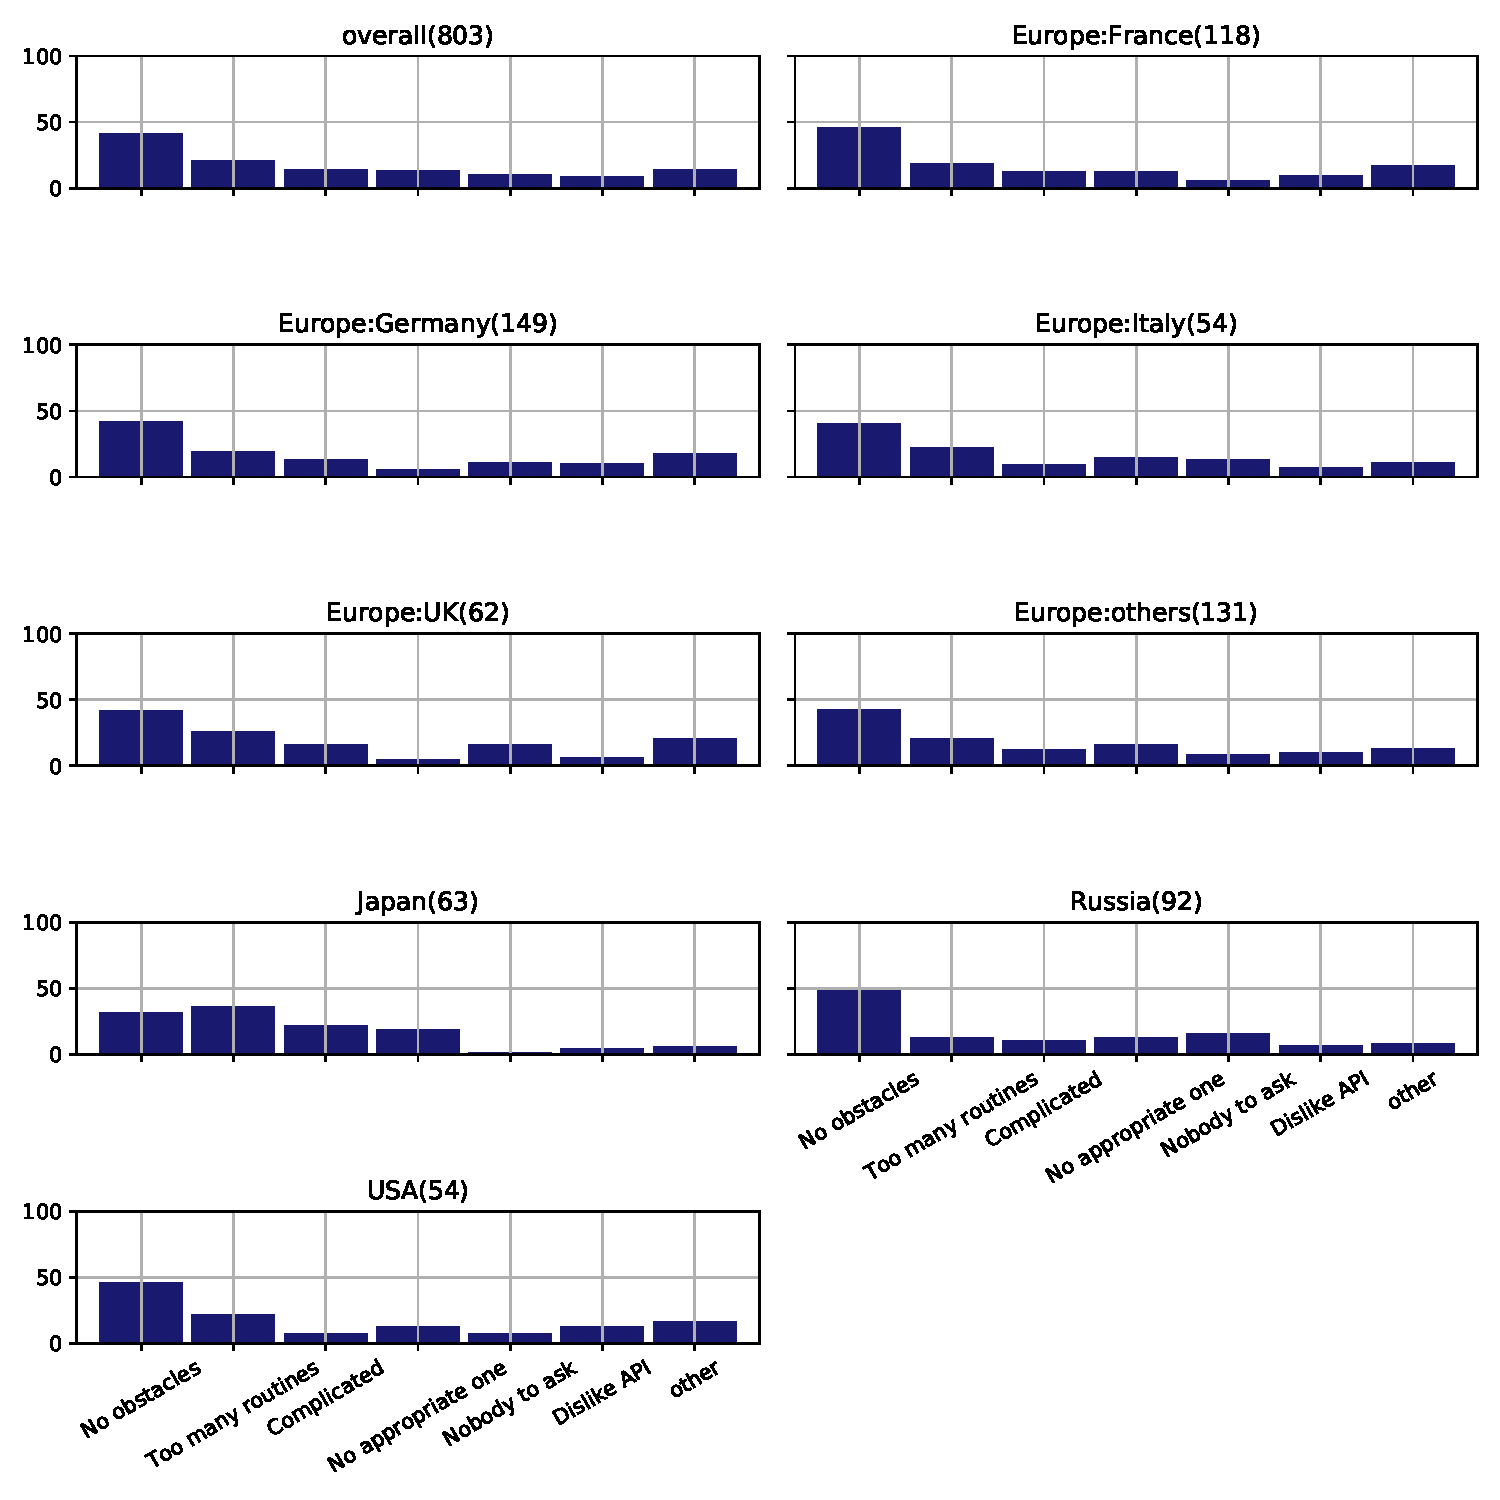
\includegraphics[width=10cm]{../pdfs/Q19.pdf}
\caption{Simple analysis: Q19}
\label{fig:Q19}
\end{center}
\end{figure}

Many Japanese think the MPI standard provides too many routines,
whereas the anser of having no obstacles dominates in the other
countries. In UK and Germany, the percentage of answer having no
appropriate lecture (, book nor tutorial) are relatively small. In UK,
however, the percentage of answer having nobody to ask is large as
well as the one of Russia.  This situation UK is very interesting. 
